\documentclass{IFES-beamer}
\usepackage{pgfplots}
\pgfplotsset{compat=1.15}
\usepackage{amssymb}
\usepackage{graphicx,xcolor}
\usepackage{color}
\definecolor{ccqqqq}{rgb}{1,0,0}
\definecolor{darkGreen}{rgb}{0,.5,0}


%%%%%%%%%%%%%%%%%%%%%%%%%%%%%%%%%%%%
%  Defini o estlo no algorithmic
%%%%%%%%%%%%%%%%%%%%%%%%%%%%%%%%%%%%%
\newcommand{\R}{\mathbb{R}}
\newcommand{\red}{\color{red}}
\newcommand{\green}{\color{green}}
\newcommand{\TODO}[1]{{{\red #1}}}
%\newcommand{\var}[1]{$#1$} %define estilo de nomes de variaveis
\newcommand{\defi}[1]{\textbf{#1}} % defini estilo ao definir algo no texto
\def\Nil{\text{NIL}}

\newcommand\circledmark{%
  \ooalign{%
    \hidewidth
    \kern-0.4ex\raisebox{-2.1ex}{\scalebox{5.5}{\textcolor{darkGreen}{\textbullet}}}
    \hidewidth\cr
    \kern-.6ex\raisebox{.6ex}{\color{white}$\checkmark$}\cr
  }%
}
\newcommand\custommark{%
  \ooalign{%
    \hidewidth
    \kern-0.4ex\raisebox{-2.1ex}{\scalebox{5.5}{\textcolor{white}{\textbullet}}}
    \hidewidth\cr
    \kern-.6ex{\color{black}$\checkmark$}\cr
  }%
}


\usepackage[Algoritmo]{algorithm}
\usepackage[noend]{algpseudocode}
\algrenewcommand\algorithmicif{\textbf{se}}
\algrenewcommand\algorithmicfor{\textbf{para}}
\algrenewcommand\algorithmicelse{\textbf{senão}}
\algrenewcommand\algorithmicwhile{\textbf{enquanto}}
\algrenewcommand\algorithmicdo{\textbf{faça}}
\algrenewcommand\algorithmicend{\textbf{fim}}
\algrenewcommand\algorithmicthen{\textbf{então}}
\algrenewcommand\algorithmicreturn{\textbf{retorne}}



\newcommand{\AlgoName}[1]{\text{\scshape #1}}

%%%%%%%%%%%%%%%%%%%%%%%%%%%%%%%%%%%%%
% Comandos de notação assintotica   %
%%%%%%%%%%%%%%%%%%%%%%%%%%%%%%%%%%%%%
\renewcommand{\O}[1]{\text{O}(#1)}
\newcommand{\OTheta}[1]{\Theta(#1)}

%%%%%%%%%%%%%%%%%%%%%%%%%%%%%%
%    Nomes de váriaveis      %
%%%%%%%%%%%%%%%%%%%%%%%%%%%%%%
\newcommand{\varname}[1]{\textit{#1}}
\newcommand{\altvarname}[1]{$#1$}
\newcommand{\node}{\textit{nó}}
\newcommand{\var}{\mathit{var}}

%%%%%%%%%%%%%%%%%%%%%%%%%%%%%%
%     Métodos de Grafos      %
%%%%%%%%%%%%%%%%%%%%%%%%%%%%%%
\newcommand{\graphCreate}{\AlgoName{novoGrafo}}
\newcommand{\graphAdd}{\AlgoName{ligueGLA}}
\newcommand{\graphDel}{\AlgoName{removaGLA}}

%%%%%%%%%%%%%%%%%%%%%%%%%%%%%%
%     Métodos de Treap       %
%%%%%%%%%%%%%%%%%%%%%%%%%%%%%%
\newcommand{\treapCreate}{\AlgoName{novoNó}}
\newcommand{\treapSearch}{\AlgoName{busca}}
\newcommand{\treapGetLast}{\AlgoName{último}}
\newcommand{\treapGetRoot}{\AlgoName{raiz}}
\newcommand{\treapOrder}{\AlgoName{ordem}}
\newcommand{\treapJoin}{\AlgoName{junta}}
\newcommand{\treapSplit}{\AlgoName{corta}}
\newcommand{\treapSplitRight}{\AlgoName{cortaDireita}}
\newcommand{\treapGetSize}{\AlgoName{tamanho}}
\newcommand{\treapGetEdgesLevel}{\AlgoName{arestasDeNível}}

\newcommand{\treapFirst}{\AlgoName{primeiro}}
\newcommand{\treapLast}{\AlgoName{último}}
\newcommand{\treapPredecessor}{\AlgoName{\AlgoName{Pred}}}    %(F, u, v)

%%%%%%%%%%%%%%%%%%%%%%%%%%%%%%
% Métodos de Euler Tour Tree %
%%%%%%%%%%%%%%%%%%%%%%%%%%%%%%
\newcommand{\ETTCreate}{\AlgoName{novoETT}}     % (v)
\newcommand{\ETTAddEdge}{\AlgoName{ligueETT}} % ($F$, $uu$, $vv$)
\newcommand{\ETTDelEdge}{\AlgoName{removaETT}} % ($F$, $uu$, $vv$)
\newcommand{\ETTQuery}{\AlgoName{conectadoETT}} % ($F$, $uu$, $vv$)
\newcommand{\ETmovetofront}{\AlgoName{movaInício}} % ($F$, $uu$)


%%%%%%%%%%%%%%%%%%%%%%%%%%%%%%%%%%
% Métodos da tabela hash         %
%%%%%%%%%%%%%%%%%%%%%%%%%%%%%%%%%%
\newcommand{\dymForestHash}{$H$}  %simbolo que identifica a matriz/hash da floresta
\newcommand{\nivel}{\AlgoName{nível}} 
\newcommand{\hashCreate}{\AlgoName{novoDicio}}     

%%%%%%%%%%%%%%%%%%%%%%%%%%%%%%%%%%
% Métodos de Florestas dinamicas %
%%%%%%%%%%%%%%%%%%%%%%%%%%%%%%%%%%
\newcommand{\dymForestCreate}{\AlgoName{novaFD}}  %(n)
\newcommand{\dymForestAddEdge}{\AlgoName{ligueFD}}    %(F, u, v)
\newcommand{\dymForestDelEdge}{\AlgoName{removaFD}}    %(F, u, v)
\newcommand{\dymForestQuery}{\AlgoName{\AlgoName{conectadoFD}}}    %(F, u, v)

%%%%%%%%%%%%%%%%%%%%%%%%%%%%%%%%%%
% Métodos de Grafos dinamicas %
%%%%%%%%%%%%%%%%%%%%%%%%%%%%%%%%%%
\newcommand{\dymGraphCreate}{\AlgoName{novoGD}}    %(n)
\newcommand{\dymGraphAddEdge}{\AlgoName{ligueGD}} %(G, u, v)
\newcommand{\dymGraphDelEdge}{\AlgoName{removaGD}} %(G, u, v)
\newcommand{\dymGraphQuery}{\AlgoName{\AlgoName{conectadoGD}}} %(G, u, v)
\newcommand{\dymGraphReplace}{\AlgoName{\AlgoName{substituaGD}}} %(G, u, v, i)
\newcommand{\dymGraphHash}{$H$}  %simbolo que identifica a matriz/hash da floresta

%%%%%%%%%%%%%%%%%%%%%%%%%%%%%%
% Métodos de Link/Cut Tree   %
%%%%%%%%%%%%%%%%%%%%%%%%%%%%%%

\newcommand{\linkcutCreate}{\AlgoName{newLCT}}
\newcommand{\linkcutDestroy}{\AlgoName{delLCT}}
\newcommand{\linkcutAddEdge}{\AlgoName{link}}    %(F, u, v)
\newcommand{\linkcutDelEdge}{\AlgoName{cut}}    %(F, u, v)
\newcommand{\linkcutEvert}{\AlgoName{\AlgoName{evert}}}    %(v)
\newcommand{\linkcutMax}{\AlgoName{\AlgoName{max}}}    %(F, u, v)
\newcommand{\linkcutMin}{\AlgoName{\AlgoName{min}}}    %(F, u, v)
\newcommand{\linkcutParent}{\AlgoName{\AlgoName{parent}}}    %(F, u, v)
\newcommand{\linkcutQuery}{\AlgoName{\AlgoName{conectadoLC}}}    %(F, u, v)
\newcommand{\linkcutWeight}{\AlgoName{\AlgoName{set weight}}}    %(F, u, v)
\newcommand{\linkcutRoot}{\AlgoName{\AlgoName{get Root}}}    %(F, u, v)

%%%%%%%%%%%%%%%%%%%%%%%%%%%%%%%%%%%%%%%
% Métodos de Link/Cut Tree com ordem  %
%%%%%%%%%%%%%%%%%%%%%%%%%%%%%%%%%%%%%%%

\newcommand{\LCOMakeOcto}{\AlgoName{Create Octo}}
\newcommand{\LCODestroyOcto}{\AlgoName{Destroy Octo}}

\newcommand{\LCOMakeNode}{\AlgoName{Make edge}}
\newcommand{\LCODestroyNode}{\AlgoName{Make edge}}
\newcommand{\LCOLink}{\AlgoName{Link}}
\newcommand{\LCOMerge}{\AlgoName{Merge}}
\newcommand{\LCOSplit}{\AlgoName{Split}}
\newcommand{\LCOCycle}{\AlgoName{Cycle}}
\newcommand{\LCOParent}{\AlgoName{\AlgoName{Parent}}}    %(F, u, v)
\newcommand{\LCORoot}{\AlgoName{Root}}
\newcommand{\LCOAddCost}{\AlgoName{Set weight}}
\newcommand{\LCOMax}{\AlgoName{\AlgoName{Find max}}}    %(F, u, v)
\newcommand{\LCOMin}{\AlgoName{\AlgoName{Find min}}}    %(F, u, v)
\newcommand{\LCOEvert}{\AlgoName{\AlgoName{Evert}}}    %(F, u, v)
\newcommand{\LCOConnected}{\AlgoName{\AlgoName{Connected}}}    %(F, u, v)
\newcommand{\LCOFindNode}{\AlgoName{Find node}}

%%%%%%%%%%%%%%%%%%%%%%%%%%%%%%
%     Métodos de MSF         %
%%%%%%%%%%%%%%%%%%%%%%%%%%%%%%
\newcommand{\MSFCreate}{\AlgoName{novoGDP}} %(n)
\newcommand{\MSFupdate}{\AlgoName{mudaPesoGDP}} %(n)
\newcommand{\MSFaddEdge}{\AlgoName{ligueGDP}}    %(G, u, v, w)
\newcommand{\MSFdelEdge}{\AlgoName{removaGDP}}    %(G, u, v)
\newcommand{\MSFweight}{\AlgoName{pesoGDP}}    %(G)

\newcommand{\dymGraphReplaceMSF}{\AlgoName{substituaGDP}} %(G, u, v, i)
\newcommand{\treapGetEdgeMinWeight}{\AlgoName{arestaMinPesoGDP}}


%%%%%%%%%%%%%%%%%%%%%%%%%%%%%%
%     Métodos de VPSP
% Verify partial sum of permutations%
%%%%%%%%%%%%%%%%%%%%%%%%%%%%%%

\newcommand{\VPSPconvert}{\AlgoName{converta}}
\newcommand{\VPSPupdate}{\AlgoName{substitua}}
\newcommand{\VPSPverify}{\AlgoName{verifique}}




% --------------------------------------------------- %
%                  Presentation info	              %
% --------------------------------------------------- %
\title[Algorit. em conexidade dinâmica]{Algoritmos para conexidade em grafos dinâmicos}
%\subtitle{Subtitle}
\author[Arthur Rodrigues]{Arthur Henrique Dias Rodrigues\\{\footnotesize sob orientação de}\\Cristina Gomes Fernandes}
\institute[IME-USP]{
  Instituto de Matemática e Estatistica\\
  USP
}
\day=22
\month=11
\year=2024
\subject{Algorit. em conexidade dinâmica} % metadata

% --------------------------------------------------- %
%                    Title + Schedule                 %
% --------------------------------------------------- %


\begin{document}
\begin{frame}
  \titlepage
\end{frame}

\begin{frame}{Sumário}
  \tableofcontents
\end{frame}

\iffalse
% --------------------------------------------------- %
%                      Presentation                   %
% --------------------------------------------------- %

\section{Problemas}
\subsection{Definições}
\begin{frame}{Problema de conexidade dinâmicas}
\begin{block}{Contexto}
\begin{itemize}
    \item $G$: grafo;
    \item $n$: número de vértices em~$G$;
    \item $F$: floresta;
    \item $u$,$v$: vértices.
    \end{itemize}
\end{block}

\begin{exampleblock}{Problema de conexidade dinâmicas}
\begin{itemize}
\item \dymGraphCreate($n$): retorna um grafo dinâmico com $n$ vértices isolados;
\item \dymGraphAddEdge($G$, $u$, $v$): adiciona aresta $uv$ a~$G$;
\item \dymGraphDelEdge($G$, $u$, $v$): remove $uv$ de $G$; e
\item \dymGraphQuery($G$, $u$, $v$): retorna verdadeiro se $u$ e~$v$ estão na mesma componente conexa de~$G$ e falso, caso contrário.
\end{itemize}
\end{exampleblock}
\end{frame}

\begin{frame}{Problemas MSF}
\boxblue{MSF: floresta maximal de peso mínimo}
\begin{block}{Grafo ponderado}
Cada aresta possui um peso associado.
\end{block}

\begin{exampleblock}{Problema de floresta maximal de peso mínimo em grafos ponderados planos dinâmicos}
\begin{itemize}
\item \MSFCreate($n$): devolve um grafo ponderado com $n$ vértices isolados;
\item \MSFaddEdge($G$, $u$, $v$, $w$): adiciona a aresta~$uv$ com peso~$w$ em~$G$;
\item \MSFdelEdge($G$, $u$, $v$): remove a aresta $uv$ de $G$; e
\item \MSFweight($G$): devolve o peso de uma MSF de $G$.
\end{itemize}
\end{exampleblock}
\end{frame}

\subsection{Resultados conhecidos}
\begin{frame}{Resultados conhecidos}
\begin{alertblock}{Limitante inferior (Patrascu e Demaine)~\cite{lowerBoundPatrascu}, 2006}
Todo algoritmo que resolve os problemas de conexidade dinâmica e de MSF dinâmica possuem consumo de tempo~$\Omega(\lg n)$.
\end{alertblock}
\begin{block}{Conexidade dinâmicas~(Holm et al.~\cite{poly_log}, 2001)}
Para árvores,~$\O{\lg n}$;\\
Grafos gerais,~$\O{\lg^2 n}$ amortizado.
\end{block}

\begin{block}{MSF~(Holm et al.~\cite{poly_log}, 2001)}
Para grafos gerais, amortizado~$\O{\lg^4 n}$.
\end{block}
\end{frame}
\fi

% --------------------------------------------------- %
%      Conexidade em florestas dinâmicas              %
% --------------------------------------------------- %
\section{Conexidade em florestas dinâmicas}
\subsection{Definição}
\begin{frame}{Conexidade em florestas dinâmicas}

\begin{exampleblock}{Problema de conexidade em florestas dinâmicas}
\begin{itemize}
\item \dymForestCreate($n$): retorna uma floresta dinâmica com $n$ vértices isolados;
\item \dymForestAddEdge($F$,$u$,$v$): adiciona $uv$ a~$F$;
\item \dymForestDelEdge($F$,$u$,$v$): remove $uv$ de $F$; e
\item \dymForestQuery($F$,$u$,$v$): retorna verdadeiro se $u$ e~$v$ estão na mesma componente conexa de~$F$ e falso, caso contrário.
\end{itemize}
\end{exampleblock}
\end{frame}

\subsection{Euler Tour Trees}

\begin{frame}{Sequência Euleriana}
\begin{figure}[htb]
\centering
\scalebox{.9}{
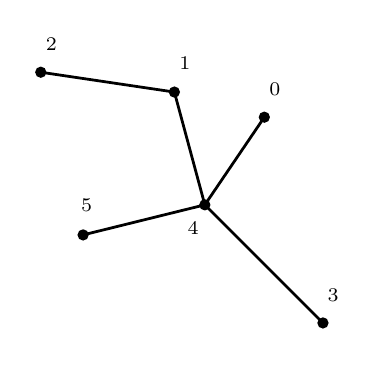
\begin{tikzpicture}[dot/.style={draw,circle,fill,inner sep=1.5pt},line width=1pt,x=1.5cm,y=1.5cm]
\clip(.5,.8) rectangle (3.3,3.5);
\draw [line width=1pt] (1.7420645075484014,2.9548225063123694)-- (0.6109449986613309,3.1228105521866865);
\draw [line width=1pt] (1.7420645075484014,2.9548225063123694)-- (2,2);
\draw [line width=1pt] (2,2)-- (0.9693194965265414,1.7453085760172875);
\draw [line width=1pt] (2,2)-- (3,1);
\draw [line width=1pt] (2,2)-- (2.5036103155119798,2.742037648204901);
\begin{scriptsize}
\draw [fill=black,bend left] (1.7420645075484014,2.9548225063123694) circle (1.5pt);
\draw[color=black] (1.8316581320147085,3.195605372065557) node {$1$};
\draw [fill=black] (0.6109449986613309,3.1228105521866865) circle (1.5pt);
\draw[color=black] (0.7005386231276353,3.363593417939874) node {$2$};
\draw [fill=black] (2,2) circle (1.5pt);
\draw[color=black] (1.9,1.8) node {$4$};
\draw [fill=black] (0.9693194965265414,1.7453085760172875) circle (1.5pt);
\draw[color=black] (1,2) node {$5$};
\draw [fill=black] (3,1) circle (1.5pt);
\draw[color=black] (3.0859688745429477,1.2357448368651927) node {$3$};
\draw [fill=black] (2.5036103155119798,2.742037648204901) circle (1.5pt);
\draw[color=black] (2.5932039399782822,2.9828205139580892) node {$0$};
\end{scriptsize}
\end{tikzpicture}
%\documentclass[border=5pt,tikz]{standalone}
%\usetikzlibrary{positioning}
%\begin{document}
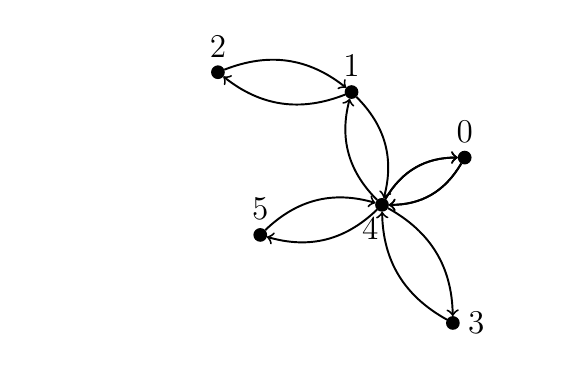
\begin{tikzpicture}[dot/.style={draw,circle,fill,inner sep=1.5pt},line width=.7pt,x=1.5cm,y=1.5cm]
\clip(-1,.8) rectangle (3.3,3.5);
\begin{scriptsize}
\node[label=above:{\large 0}] (r0) at (2.7,2.4) [dot] {};

\node[label=above:{\large 1}] (r1) at (1.7420645075484014,2.9548225063123694) [dot] {};
%\draw[color=black] (1.8316581320147085,3.195605372065557) node {$1$};


\node[label=above:{\large 2}] (r2) at (0.6109449986613309,3.1228105521866865) [dot] {};
%\draw[color=black] (0.7005386231276353,3.363593417939874) node {$2$};

\node[label=right:{\large 3}] (r3) at (2.6,1) [dot] {};
%\draw[color=black] (2.6,1.2357448368651927) node {$3$};

\node (r4) at (2,2) [dot] {};
\draw[color=black] (1.9,1.8) node {{\large 4}};

\node[label=above:{\large 5}] (r5) at (0.9693194965265414,1.7453085760172875) [dot] {};
%\draw[color=black] (1,2) node {$5$};

\draw[->] (r0) to[bend left] (r4);
\draw[->] (r4) to[bend left] (r0);

\draw[->] (r3) to[bend left] (r4);
\draw[->] (r4) to[bend left] (r3);

\draw[->] (r5) to[bend left] (r4);
\draw[->] (r4) to[bend left] (r5);

\draw[->] (r1) to[bend left] (r4);
\draw[->] (r4) to[bend left] (r1);

\draw[->] (r0) to[bend left] (r4);
\draw[->] (r4) to[bend left] (r0);

\draw[->] (r1) to[bend left] (r2);
\draw[->] (r2) to[bend left] (r1);

\end{scriptsize}
\end{tikzpicture}
%\end{document}

	}
\end{figure}
\begin{center}
{\large 30~00~04~41~12~22~21~11~14~44~45~55~54~40~03~33}
\end{center}
\end{frame}

\begin{frame}{Euler Tour Trees}
\begin{figure}[htb]
\centering
\scalebox{.7}{
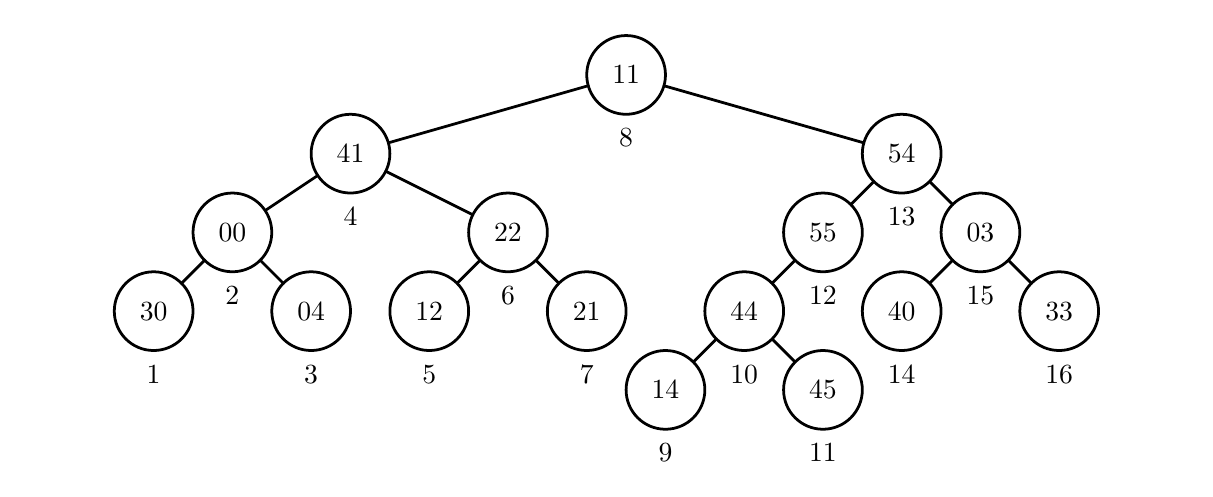
\begin{tikzpicture}[line cap=round,line join=round,x=1cm,y=1cm]
\clip(-.6,-1) rectangle (14.1,4.6);
\draw [line width=1pt] (1,1) circle (0.5cm);
\draw [line width=1pt] (2,2) circle (0.5cm);
\draw [line width=1pt] (3,1) circle (0.5cm);
\draw [line width=1pt] (5.5,2) circle (0.5cm);
\draw [line width=1pt] (6.5,1) circle (0.5cm);
\draw [line width=1pt] (3.5,3) circle (0.5cm);
\draw [line width=1pt] (7,4) circle (0.5cm);
\draw [line width=1pt] (10.5,3) circle (0.5cm);
\draw [line width=1pt] (9.5,2) circle (0.5cm);
\draw [line width=1pt] (8.5,1) circle (0.5cm);
\draw [line width=1pt] (11.5,2) circle (0.5cm);
\draw [line width=1pt] (10.5,1) circle (0.5cm);
\draw [line width=1pt] (12.5,1) circle (0.5cm);
\draw [line width=1pt] (4.5,1) circle (0.5cm);
\draw [line width=1pt] (7.5,0) circle (0.5cm);
\draw [line width=1pt] (9.5,0) circle (0.5cm);
\draw [line width=1pt] (1.3535533905932737,1.3535533905932737)-- (1.646446609406726,1.646446609406726);
\draw [line width=1pt] (2.353553390593274,1.646446609406726)-- (2.646446609406726,1.353553390593274);
i%\draw [line width=1pt] (2.646446609406726,0.646446609406726)-- (2.353553390593274,0.35355339059327395);
\draw [line width=1pt] (2.416025147168923,2.2773500981126156)-- (3.0839748528310773,2.722649901887385);
\draw [line width=1pt] (3.947213595499958,2.776393202250021)-- (5.052786404500042,2.223606797749979);
\draw [line width=1pt] (5.146446609406726,1.646446609406726)-- (4.853553390593274,1.353553390593274);
\draw [line width=1pt] (5.853553390593274,1.646446609406726)-- (6.146446609406726,1.353553390593274);
\draw [line width=1pt] (10.01923802617959,3.137360563948689)-- (7.480761973820412,3.8626394360513108);
\draw [line width=1pt] (6.519238026179588,3.8626394360513108)-- (3.9807619738204116,3.137360563948689);
\draw [line width=1pt] (10.146446609406727,2.646446609406727)-- (9.853553390593273,2.353553390593273);
\draw [line width=1pt] (9.146446609406727,1.646446609406727)-- (8.853553390593273,1.353553390593273);
\draw [line width=1pt] (8.146446609406727,0.6464466094067269)-- (7.853553390593274,0.35355339059327395);
\draw [line width=1pt] (8.853553390593273,0.6464466094067269)-- (9.146446609406727,0.35355339059327306);
\draw [line width=1pt] (10.853553390593273,1.353553390593273)-- (11.146446609406727,1.646446609406727);
\draw [line width=1pt] (11.146446609406727,2.353553390593273)-- (10.853553390593273,2.646446609406727);
\draw [line width=1pt] (11.853553390593273,1.646446609406727)-- (12.146446609406727,1.353553390593273);


\draw[color=black] (1,1) node {$30$};
\draw[color=black] (1,.2) node {1};
\draw[color=black] (2,2) node {$00$};
\draw[color=black] (2,1.2) node {2};
\draw[color=black] (3,1) node {$04$};
\draw[color=black] (3,.2) node {3};
\draw[color=black] (3.5,3) node {$41$};
\draw[color=black] (3.5,2.2) node {4};
\draw[color=black] (4.5,1) node {$12$};
\draw[color=black] (4.5,.2) node {5};
\draw[color=black] (5.5,2) node {$22$};
\draw[color=black] (5.5,1.2) node {6};
\draw[color=black] (6.5,1) node {$21$};
\draw[color=black] (6.5,.2) node {7};
\draw[color=black] (7,4) node {$11$};
\draw[color=black] (7,3.2) node {8};
\draw[color=black] (7.5,0) node {$14$};
\draw[color=black] (7.5,-.8) node {9};
\draw[color=black] (8.5,1) node {$44$};
\draw[color=black] (8.5,.2) node {10};
\draw[color=black] (9.5,0) node {$45$};
\draw[color=black] (9.5,-.8) node {11};
\draw[color=black] (9.5,2) node {$55$};
\draw[color=black] (9.5,1.2) node {12};
\draw[color=black] (10.5,3) node {$54$};
\draw[color=black] (10.5,2.2) node {13};
\draw[color=black] (10.5,1) node {$40$};
\draw[color=black] (10.5,.2) node {14};
\draw[color=black] (11.5,2) node {$03$};
\draw[color=black] (11.5,1.2) node {15};
\draw[color=black] (12.5,1) node {$33$};
\draw[color=black] (12.5,.2) node {16};


\end{tikzpicture}
}
\end{figure}
\begin{center}
{\large 30~00~04~41~12~22~21~11~14~44~45~55~54~40~03~33}
\end{center}
\end{frame}



\begin{frame}{Chaves implícitas}
\begin{figure}[htb]
\scalebox{.7}{
\centering
\begin{tikzpicture}[line cap=round,line join=round,>=triangle 45,x=1cm,y=1cm]
\clip(-.6,-1) rectangle (14.1,4.6);
\draw [line width=1pt] (1,1) circle (0.5cm);
\draw [line width=1pt] (2,2) circle (0.5cm);
\draw [line width=1pt] (3,1) circle (0.5cm);
\draw [line width=1pt] (5.5,2) circle (0.5cm);
\draw [line width=1pt] (6.5,1) circle (0.5cm);
\draw [line width=1pt] (3.5,3) circle (0.5cm);
\draw [line width=1pt] (7,4) circle (0.5cm);
\draw [line width=1pt] (10.5,3) circle (0.5cm);
\draw [line width=1pt] (9.5,2) circle (0.5cm);
\draw [line width=1pt] (8.5,1) circle (0.5cm);
\draw [line width=1pt] (11.5,2) circle (0.5cm);
\draw [line width=1pt] (10.5,1) circle (0.5cm);
\draw [line width=1pt] (12.5,1) circle (0.5cm);
\draw [line width=1pt] (4.5,1) circle (0.5cm);
\draw [line width=1pt] (7.5,0) circle (0.5cm);
\draw [line width=1pt] (9.5,0) circle (0.5cm);
\draw [line width=1pt] (1.3535533905932737,1.3535533905932737)-- (1.646446609406726,1.646446609406726);
\draw [line width=1pt] (2.353553390593274,1.646446609406726)-- (2.646446609406726,1.353553390593274);
i%\draw [line width=1pt] (2.646446609406726,0.646446609406726)-- (2.353553390593274,0.35355339059327395);
\draw [line width=1pt] (2.416025147168923,2.2773500981126156)-- (3.0839748528310773,2.722649901887385);
\draw [line width=1pt] (3.947213595499958,2.776393202250021)-- (5.052786404500042,2.223606797749979);
\draw [line width=1pt] (5.146446609406726,1.646446609406726)-- (4.853553390593274,1.353553390593274);
\draw [line width=1pt] (5.853553390593274,1.646446609406726)-- (6.146446609406726,1.353553390593274);
\draw [line width=1pt] (10.01923802617959,3.137360563948689)-- (7.480761973820412,3.8626394360513108);
\draw [line width=1pt] (6.519238026179588,3.8626394360513108)-- (3.9807619738204116,3.137360563948689);
\draw [line width=1pt] (10.146446609406727,2.646446609406727)-- (9.853553390593273,2.353553390593273);
\draw [line width=1pt] (9.146446609406727,1.646446609406727)-- (8.853553390593273,1.353553390593273);
\draw [line width=1pt] (8.146446609406727,0.6464466094067269)-- (7.853553390593274,0.35355339059327395);
\draw [line width=1pt] (8.853553390593273,0.6464466094067269)-- (9.146446609406727,0.35355339059327306);
\draw [line width=1pt] (10.853553390593273,1.353553390593273)-- (11.146446609406727,1.646446609406727);
\draw [line width=1pt] (11.146446609406727,2.353553390593273)-- (10.853553390593273,2.646446609406727);
\draw [line width=1pt] (11.853553390593273,1.646446609406727)-- (12.146446609406727,1.353553390593273);


\draw[color=black] (1,1) node {$30$};
\draw[color=black] (1,.2) node {1};
\draw[color=black] (2,2) node {$00$};
\draw[color=black] (2,1.2) node {3};
\draw[color=black] (3,1) node {$04$};
\draw[color=black] (3,.2) node {1};
\draw[color=black] (3.5,3) node {$41$};
\draw[color=black] (3.5,2.2) node {7};
\draw[color=black] (4.5,1) node {$12$};
\draw[color=black] (4.5,.2) node {1};
\draw[color=black] (5.5,2) node {$22$};
\draw[color=black] (5.5,1.2) node {3};
\draw[color=black] (6.5,1) node {$21$};
\draw[color=black] (6.5,.2) node {1};
\draw[color=black] (7,4) node {$11$};
\draw[color=black] (7,3.2) node {16};
\draw[color=black] (7.5,0) node {$14$};
\draw[color=black] (7.5,-.8) node {1};
\draw[color=black] (8.5,1) node {$44$};
\draw[color=black] (8.5,.2) node {3};
\draw[color=black] (9.5,0) node {$45$};
\draw[color=black] (9.5,-.8) node {1};
\draw[color=black] (9.5,2) node {$55$};
\draw[color=black] (9.5,1.2) node {4};
\draw[color=black] (10.5,3) node {$54$};
\draw[color=black] (10.5,2.2) node {8};
\draw[color=black] (10.5,1) node {$40$};
\draw[color=black] (10.5,.2) node {1};
\draw[color=black] (11.5,2) node {$03$};
\draw[color=black] (11.5,1.2) node {3};
\draw[color=black] (12.5,1) node {$33$};
\draw[color=black] (12.5,.2) node {1};


\end{tikzpicture}
}
\end{figure}
\begin{center}
{\large 30~00~04~41~12~22~21~11~14~44~45~55~54~40~03~33}
\end{center}
\end{frame}


\begin{frame}{Biblioteca de Euler Tour Trees}
\begin{exampleblock}{Biblioteca de Euler Tour Trees}
\begin{itemize}
\item  \treapCreate($u$, $v$): retorna uma ABB com um único nó com valor uv;
\item \treapJoin($T$, $R$): junta as ABBs $T$ e $R$ concatenando as sequências Eulerianas armazenada nelas e retorna a raiz da árvore resultante.
\item \treapSplit($\node$): corta a ABB que contém um nó~$\node$ em três ABBs. A primeira ABB contém todos os nós com chave estritamente menor do que a chave de~$\node$, a segunda contém somente~$\node$ e a última contém todos os nós com chave estritamente maior do que a chave de~$\node$. Essa rotina retorna as raízes dessas três ABBs; e
\item \treapGetRoot($x$): retorna a raiz da ABB que contém $x$;
\end{itemize}
\end{exampleblock}
\boxpurple{\centering  \treapCreate{}:~$\O{1}$.\\ As demais operações :~$\O{\lg n}$.}
\end{frame}

\begin{frame}{Tabela de símbolos}
\boxblue{
\centering
Associa $(u,v) \rightarrow uv$.
}
\begin{exampleblock}{Biblioteca de tabela de símbolos}
\begin{itemize}
    \item $F \gets \hashCreate(n)$: cria e retorna um dicionário~$F$ para uma floresta dinâmica com~$n$ vértices;
    \item $F[u,v] \gets uv$: insere o nó que contém $uv$, com chave $(u,v)$ e valor associado~$uv$ na tabela~$F$.
    Se o par~$(u,v)$ já estiver presente no dicionário, então seu valor associado é substituído por~$uv$;
    \item $F[u,v] \gets \Nil{}$: remove o nó associado a~$(u,v)$ e seu valor associado do dicionário~$F$;
    \item $\var{} \gets F[u,v]$: atribui o valor associado à chave~$(u,v)$ à variável~$\var$;
	Caso a chave~$(u,v)$ não esteja presente em~$F$, atribui~$\Nil$ a~$\var{} $.
\end{itemize}
\end{exampleblock}
\boxpurple{
\centering
Consumo esperado~$\O{1}$ por rotina~\cite{CLRS}.
}
\end{frame}

\begin{frame}{Implementação da interface de floresta dinâmica}
\begin{algorithm}[H]
\caption{\dymForestCreate($n$)}
\label{Algo:dymForestCreate}
\begin{algorithmic}[1]
\State $F~\gets~\hashCreate(n)$
\For {$v$ $\gets$ 1 até $n$}\label{Algo:dymForestCreate:for}
\State $F[v,v]~\gets$ \treapCreate($v$, $v$)
\EndFor
\State \Return $F$
\end{algorithmic}
\end{algorithm}
\begin{algorithm}[H]
\caption{\dymForestQuery($F$, $u$, $v$)}
\label{Algo:dymForestQuery}
\begin{algorithmic}[1]
\State \varname{uu} $\gets$ $F[u,u]$
\State $vv$ $\gets$ $F[v,v]$
\State \Return \treapGetRoot(\varname{uu}) = \treapGetRoot($vv$)
\end{algorithmic}
\end{algorithm}
\boxpurple{
\centering
~~~~~\dymForestCreate{} : $\O{n}$\\
\dymForestQuery{}  : $\O{\lg n}$
}
\end{frame}

\begin{frame}{Implementação da interface de floresta dinâmica}
\begin{algorithm}[H]
\caption{\ETmovetofront($F$,$u$)}
\label{Algo:ETmovetofront}
\begin{algorithmic}[1]
\State \varname{uu} $\gets$ $F[u,u]$\label{Algo:ETmovetofront:1}
\State $A$, \varname{uu}, $B$ $\gets$ \treapSplit(\varname{uu})\label{Algo:ETmovetofront:2}
\State \Return \treapJoin(\varname{uu}, $B$, $A$)\label{Algo:ETmovetofront:3}
\end{algorithmic}
\end{algorithm}
\begin{algorithm}[H]
\caption{\dymForestAddEdge($F$,$u$,$v$)}
\label{Algo:dymForestAddEdge}
\begin{algorithmic}[1]
\State $U$ $\gets$ \ETmovetofront($F$, $u$)
\State $V$ $\gets$ \ETmovetofront($F$, $v$)
\State $uv$ $\gets$ \treapCreate($u$, $v$)
\State $vu$ $\gets$ \treapCreate($v$, $u$)
\State $F[u,v]$ $\gets$ $uv$
\State $F[v,u]$ $\gets$ $vu$
\State \treapJoin($U$, $uv$, $V$, $vu$)
\end{algorithmic}
\end{algorithm}
\boxpurple{
\centering
\dymForestAddEdge{}  : $\O{\lg n}$\\
\ETmovetofront{}  : $\O{\lg n}$
}
\end{frame}

\begin{frame}{Implementação da interface de floresta dinâmica}
\begin{algorithm}[H]
\caption{\dymForestDelEdge($F$, $u$, $v$)}
\label{Algo:dymForestDelEdge}
\begin{algorithmic}[1]
\State $uv$ $\gets$ $F[u,v]$\label{Algo:dymForestDelEdge:1}
\State $vu$ $\gets$ $F[v,u]$\label{Algo:dymForestDelEdge:2}
\State $A$, $uv$, $B$ $\gets$ \treapSplit($uv$)\label{Algo:dymForestDelEdge:3}
\State \treapJoin($B$, $A$)\label{Algo:dymForestDelEdge:4}
\State \treapSplit($vu$)\label{Algo:dymForestDelEdge:5}
\State $F[u,v]$ $\gets$ $\Nil{}$\label{Algo:dymForestDelEdge:6}
\State $F[v,u]$ $\gets$ $\Nil{}$\label{Algo:dymForestDelEdge:7}
\end{algorithmic}
\end{algorithm}
\boxpurple{
\centering
\dymForestDelEdge{}  : $\O{\lg n}$
}
\end{frame}

\subsection{Treaps}
\begin{frame}{Uma treap imersa no plano cartesiano.}
\boxblue{
\centering
Cada nó de uma treap possui um par ordenado \textbf{(chave, prioridade)}
}
\begin{figure}[htb]
\centering
\scalebox{.45}{
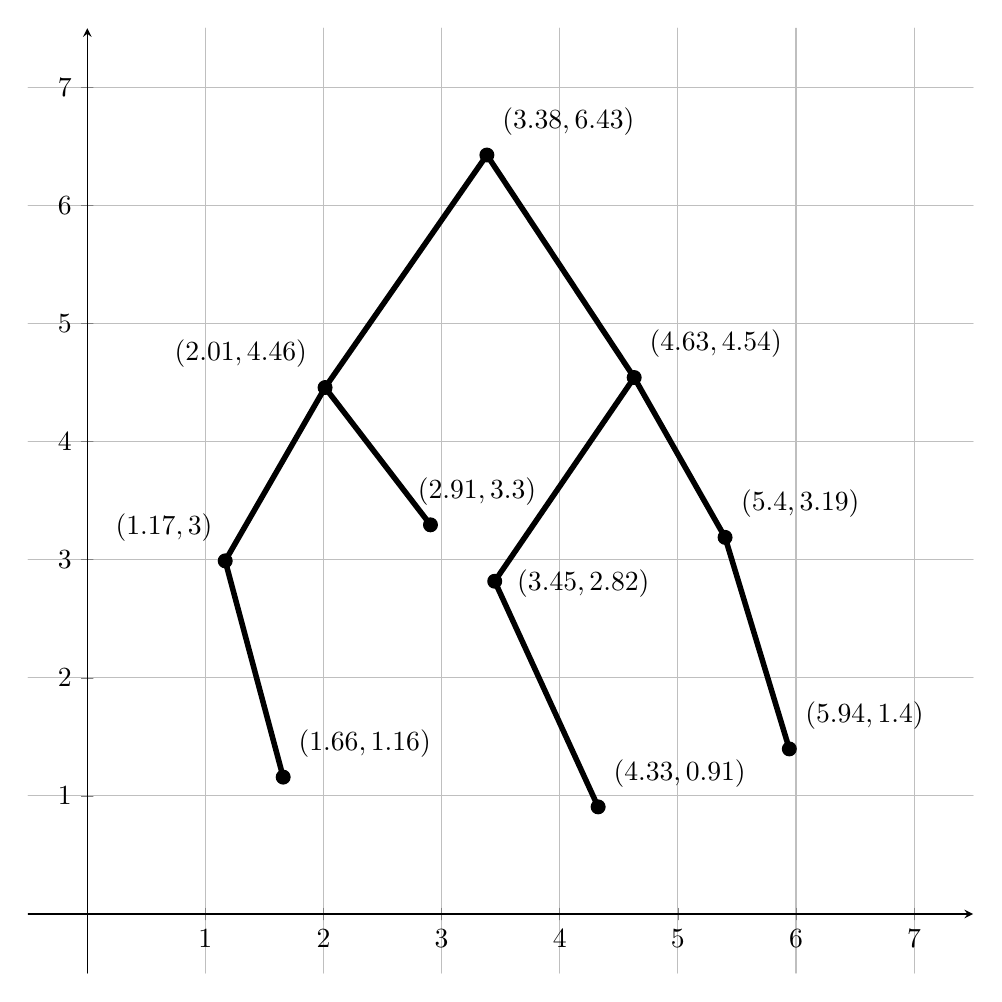
\begin{tikzpicture}[line cap=round,line join=round,x=1cm,y=1cm]
\begin{axis}[
x=1.5cm,y=1.5cm,
axis lines=middle,
ymajorgrids=true,
xmajorgrids=true,
xmin=-.5,
xmax=7.5,
ymin=-.5,
ymax=7.5,
xtick={-3,-2,...,16},
ytick={-1,0,...,10},]
\clip(-1,-1) rectangle (16.11970291004026,10.724908935002318);
\draw [line width=2pt] (3.383319601128083,6.426379568244459)-- (2.0132670659467835,4.457693392208796);
\draw [line width=2pt] (3.383319601128083,6.426379568244459)-- (4.630423800125734,4.5424562038011995);
\draw [line width=2pt] (2.0132670659467835,4.457693392208796)-- (1.1677195880152356,2.990209488027528);
\draw [line width=2pt] (2.0132670659467835,4.457693392208796)-- (2.9057052270438763,3.295352004803549);
\draw [line width=2pt] (4.630423800125734,4.5424562038011995)-- (3.449654930862001,2.8177376307193422);
\draw [line width=2pt] (4.630423800125734,4.5424562038011995)-- (5.399913625039178,3.189215477229281);
\draw [line width=2pt] (3.449654930862001,2.8177376307193422)-- (4.325281283349713,0.9072801343825158);
\draw [line width=2pt] (5.399913625039178,3.189215477229281)-- (5.943863328857303,1.3981615744135059);
\draw [line width=2pt] (1.1677195880152356,2.990209488027528)-- (1.6586010280462258,1.1593543873714025);
\begin{scriptsize}
\draw [fill=black] (3.383319601128083,6.426379568244459) circle (2.5pt);
\draw[color=black] (4.073207030360826,6.711621486100305) node {$(3.38, 6.43)$};
\draw [fill=black] (2.0132670659467835,4.457693392208796) circle (2.5pt);
\draw[color=black] (1.3,4.748095725976344) node {$(2.01, 4.46)$};
\draw [fill=black] (4.630423800125734,4.5424562038011995) circle (2.5pt);
\draw[color=black] (5.320311229358477,4.827698121657045) node {$(4.63, 4.54)$};
\draw [fill=black] (1.1677195880152356,2.990209488027528) circle (2.5pt);
\draw[color=black] (.65,3.275451405883374) node {$(1.17, 3)$};
\draw [fill=black] (2.9057052270438763,3.295352004803549) circle (2.5pt);
\draw[color=black] (3.3,3.5805939226593946) node {$(2.91, 3.3)$};
\draw [fill=black] (3.449654930862001,2.8177376307193422) circle (2.5pt);
\draw[color=black] (4.2,2.8) node {$(3.45, 2.82)$};
\draw [fill=black] (5.399913625039178,3.189215477229281) circle (2.5pt);
\draw[color=black] (6.036732790484788,3.4744573950851265) node {$(5.4, 3.19)$};
\draw [fill=black] (4.325281283349713,0.9072801343825158) circle (2.5pt);
\draw[color=black] (5.015168712582456,1.1925220522383615) node {$(4.33, 0.91)$};
\draw [fill=black] (5.943863328857303,1.3981615744135059) circle (2.5pt);
\draw[color=black] (6.580682494302912,1.6834034922693517) node {$(5.94, 1.4)$};
\draw [fill=black] (1.6586010280462258,1.1593543873714025) circle (2.5pt);
\draw[color=black] (2.3484884572789686,1.4445963052272481) node {$(1.66, 1.16)$};
\end{scriptsize}
\end{axis}
\end{tikzpicture}}
\end{figure}
\end{frame}

% --------------------------------------------------- %
%      Conexidade em grafos dinâmicos              %
% --------------------------------------------------- %
\section{Conexidade em grafos dinâmicos}
\subsection{Definição}
\begin{frame}{Conexidade em grafos dinâmicos}
\begin{exampleblock}{Conexidade em grafos dinâmicos}
\begin{itemize}
\item \dymGraphCreate($n$): cria um grafo dinâmico com $n$ vértices isolados;
\item \dymGraphAddEdge($G$, $u$, $v$): adiciona a aresta $uv$ ao grafo dinâmico $G$;
\item \dymGraphDelEdge($G$, $u$, $v$): remove a aresta $uv$ de $G$; e
\item \dymGraphQuery($G$, $u$, $v$): retorna verdadeiro se $u$ e $v$ estão na mesma componente conexa de $G$ e falso, caso contrário.
\end{itemize}
\end{exampleblock}

\end{frame}

\begin{frame}{Ideia inicial}
\begin{block}{Manteremos}
\begin{itemize}
    \item floresta maximal dinâmica~$F$ de~$G$; e
    \item um grafo~$R$ = $G-F$
\end{itemize}
\end{block}

\begin{exampleblock}{Lista de adjacências}
\begin{itemize}
    \item \graphCreate($n$): devolve a representação por listas de adjacências de um grafo com~$n$ vértices isolados.
    \item \graphAdd($G$, $u$, $v$): adiciona $u$ na lista de adjacências de $v$ em $G$ e vice-versa.
    \item \graphDel($G$, $u$, $v$): remove $u$ da lista de adjacências de $v$ em $G$ e vice-versa.
\end{itemize}
\end{exampleblock}
\boxpurple{
\centering
~~~~~~\graphCreate{} : $\O{n}$\\
\graphAdd{}  : $\O{1}$\\
\graphDel{}  : $\O{1}$\\
}
\end{frame}


\begin{frame}{Ideia inicial}
\begin{algorithm}[H]
\caption{\dymGraphQuery($G$, $u$, $v$)}
\label{Algo:dymGraphQuery}
\begin{algorithmic}[1]
\State \Return \dymForestQuery($G$.$F$, $u$, $v$)
\end{algorithmic}
\end{algorithm}

\begin{algorithm}[H]
\caption{\dymGraphAddEdge($G$, $u$, $v$)}
\label{Algo:dymGraphAddEdge}
\begin{algorithmic}[1]
\If {\dymForestQuery($G.F$, $u$, $v$)}
\State \graphAdd($G$.$R$, $u$, $v$)
\Else 
\State \dymForestAddEdge($G.F$, $u$, $v$)
\EndIf
\end{algorithmic}
\end{algorithm}


\boxpurple{
\dymGraphQuery{} : $\O{\lg n}$\\
\dymGraphAddEdge{}  : $\O{\lg^2 n}$ amortizado\TODO{!!}
}
\end{frame}



\begin{frame}{Remoção de arestas}
\begin{block}{Estrutura de níveis}
\begin{itemize}
    \item Cada aresta possui um \defi{nível}, que é um inteiro entre~$1$ e $\lceil \log n \rceil$;
    \item Arestas serão inseridas no nível~$\lceil \log n \rceil$;
    \item O nível de uma aresta pode diminuir, mas nunca aumentar. 
\end{itemize}
\end{block}
\begin{block}{Estrutura}
$G_{\leqslant i}$: grafo com arestas de nível $\leqslant i$. Para cada camada $i$, manteremos:
\begin{itemize}
    \item $F_{\leqslant i}$: floresta maximal  de~$G_{\leqslant i}$; e
    \item $R_i$: arestas de nível~$i \notin F_{\leqslant i}$.
\end{itemize}
\end{block}
\begin{block}{Invariantes}
\begin{itemize}
    \item $F_{\leqslant i} \subseteq F_{\leqslant i+1}$, para cada $1\leqslant i \leqslant \lceil \log n \rceil-1$;
    \item $F_{\leqslant i}$ é uma floresta maximal de~$G_{\leqslant i}$; e
    \item Cada componente de $F_i$ possui menos do que $2^i$ arestas.
\end{itemize}
\end{block}
\end{frame}

\begin{frame}{Implementações}
\begin{exampleblock}{Adaptações}
\centering
$G.F\rightarrow G.F_{\leqslant \lceil \log n \rceil}$\\
$G.R\rightarrow G.R_{\leqslant \lceil \log n \rceil}$
\end{exampleblock}
\begin{algorithm}[H]
\caption{\dymGraphDelEdge($G$, $u$, $v$)}
\label{Algo:dymGraphDelEdge}
\begin{algorithmic}[1]
\State $i$ $\gets$ \nivel[$u,v$]
\State \nivel[$u,v$] $\gets$ $\Nil$
\If {$uv$ $\in G.F_{\leqslant\lceil \lg n \rceil}$}\label{Algo:dymGraphDelEdge:linha:if}
\For {$j$ $\gets$ $i$ até $\lceil \lg n \rceil$}\label{linha2}
\State \dymForestDelEdge($G$.$F_j$, $u$, $v$)
\EndFor
\State \dymGraphReplace($G$, $u$, $v$, $i$)
\Else
  \State \graphDel($G$.$R_i$, $u$, $v$)\label{Algo:dymGraphDelEdge:linha:removeLA}
\EndIf
\end{algorithmic}
\end{algorithm}
\boxpurple{
\centering
\dymGraphDelEdge{}  : $\O{\lg^2 n}$ amortizado.
}
\end{frame}

\begin{frame}{Estrutura de níveis}
\begin{figure}[htb]
\scalebox{.5}{
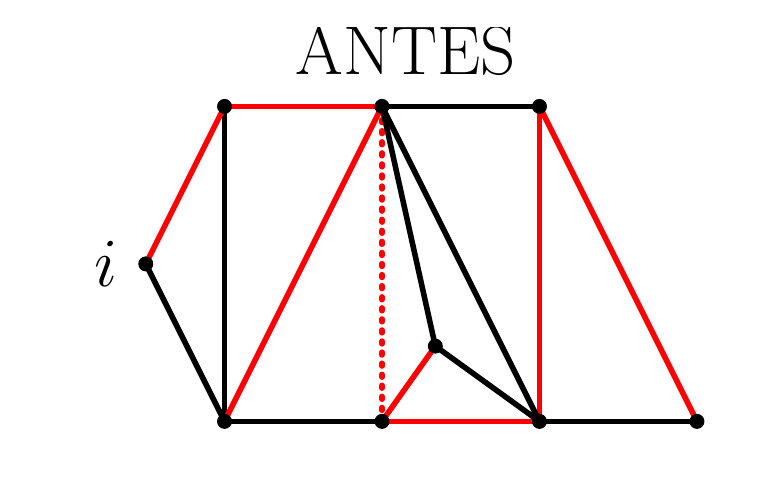
\begin{tikzpicture}[line cap=round,line join=round,x=1cm,y=1cm]
\clip(-1.5,-.5) rectangle (7.5,5);
\draw (3.3,4.7) node {{\Huge ANTES}};
\draw (-.5,2) node {{\Huge $i$}};
\draw [line width=2pt,color=ccqqqq] (3,0)-- (3.677138935355088,0.9555967043150745);
\draw [line width=2pt] (3,0)-- (1,0);
\draw [line width=2pt] (1,0)-- (1,4);
\draw [line width=2pt] (1,0)-- (0,2);
\draw [line width=2pt,color=ccqqqq,dash pattern=on 1pt off 3pt] (3,0)-- (3,4);
\draw [line width=2pt,color=ccqqqq] (3,0)-- (5,0);
\draw [line width=2pt,color=ccqqqq] (5,0)-- (5,4);
\draw [line width=2pt,color=ccqqqq] (1,4)-- (3,4);
\draw [line width=2pt] (3,4)-- (5,0);
\draw [line width=2pt] (3.677138935355088,0.9555967043150745)-- (5,0);
\draw [line width=2pt] (5,4)-- (3,4);
\draw [line width=2pt,color=ccqqqq] (1,4)-- (0,2);
\draw [line width=2pt,color=ccqqqq] (1,0)-- (3,4);
\draw [line width=2pt] (3,4)-- (3.677138935355088,0.9555967043150745);
\draw [line width=2pt,color=ccqqqq] (5,4)-- (7,0);
\draw [line width=2pt] (7,0)-- (5,0);
\begin{scriptsize}
\draw [fill=black] (3,0) circle (2.5pt);
\draw [fill=black] (3.677138935355088,0.9555967043150745) circle (2.5pt);
\draw [fill=black] (1,0) circle (2.5pt);
\draw [fill=black] (1,4) circle (2.5pt);
\draw [fill=black] (0,2) circle (2.5pt);
\draw [fill=black] (3,4) circle (2.5pt);
\draw [fill=black] (5,0) circle (2.5pt);
\draw [fill=black] (5,4) circle (2.5pt);
\draw [fill=black] (7,0) circle (2.5pt);
\end{scriptsize}
\end{tikzpicture}

\begin{tikzpicture}[line cap=round,line join=round,x=1cm,y=1cm]
\clip(0,-.5) rectangle (5,4.5);
\end{tikzpicture}
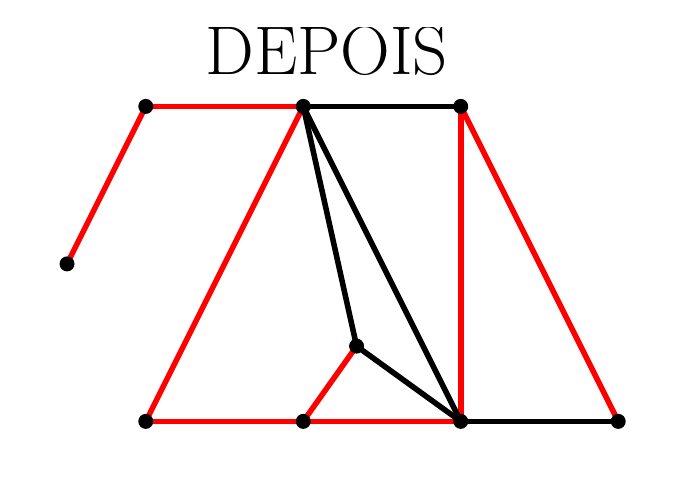
\begin{tikzpicture}[line cap=round,line join=round,x=1cm,y=1cm]
\clip(-.5,-.5) rectangle (7.5,5);
\draw (3.3,4.7) node {{\Huge DEPOIS}};
\draw [line width=2pt,color=ccqqqq] (3,0)-- (3.677138935355088,0.9555967043150745);
\draw [line width=2pt,color=ccqqqq] (3,0)-- (1,0);
\draw [line width=2pt,color=ccqqqq] (3,0)-- (5,0);
\draw [line width=2pt,color=ccqqqq] (5,0)-- (5,4);
\draw [line width=2pt,color=ccqqqq] (1,4)-- (3,4);
\draw [line width=2pt] (3,4)-- (5,0);
\draw [line width=2pt] (3.677138935355088,0.9555967043150745)-- (5,0);
\draw [line width=2pt] (5,4)-- (3,4);
\draw [line width=2pt,color=ccqqqq] (1,4)-- (0,2);
\draw [line width=2pt,color=ccqqqq] (1,0)-- (3,4);
\draw [line width=2pt] (3,4)-- (3.677138935355088,0.9555967043150745);
\draw [line width=2pt,color=ccqqqq] (5,4)-- (7,0);
\draw [line width=2pt] (7,0)-- (5,0);
\begin{scriptsize}
\draw [fill=black] (3,0) circle (2.5pt);
\draw [fill=black] (3.677138935355088,0.9555967043150745) circle (2.5pt);
\draw [fill=black] (1,0) circle (2.5pt);
\draw [fill=black] (1,4) circle (2.5pt);
\draw [fill=black] (0,2) circle (2.5pt);
\draw [fill=black] (3,4) circle (2.5pt);
\draw [fill=black] (5,0) circle (2.5pt);
\draw [fill=black] (5,4) circle (2.5pt);
\draw [fill=black] (7,0) circle (2.5pt);
\end{scriptsize}
\end{tikzpicture}
}
\end{figure}
\begin{figure}[htb]
\scalebox{.5}{
\begin{tikzpicture}[line cap=round,line join=round,x=1cm,y=1cm]
\clip(-2,-.5) rectangle (7.5,4.5);
\draw (-1,2) node {{\Huge $i-1$}};
\begin{scriptsize}
\draw [fill=black] (3,0) circle (2.5pt);
\draw [fill=black] (3.677138935355088,0.9555967043150745) circle (2.5pt);
\draw [fill=black] (1,0) circle (2.5pt);
\draw [fill=black] (1,4) circle (2.5pt);
\draw [fill=black] (0,2) circle (2.5pt);
\draw [fill=black] (3,4) circle (2.5pt);
\draw [fill=black] (5,0) circle (2.5pt);
\draw [fill=black] (5,4) circle (2.5pt);
\draw [fill=black] (7,0) circle (2.5pt);
\end{scriptsize}
\end{tikzpicture}

\begin{tikzpicture}[line cap=round,line join=round,x=1cm,y=1cm]
\clip(0,-.5) rectangle (5,4.5);
\end{tikzpicture}
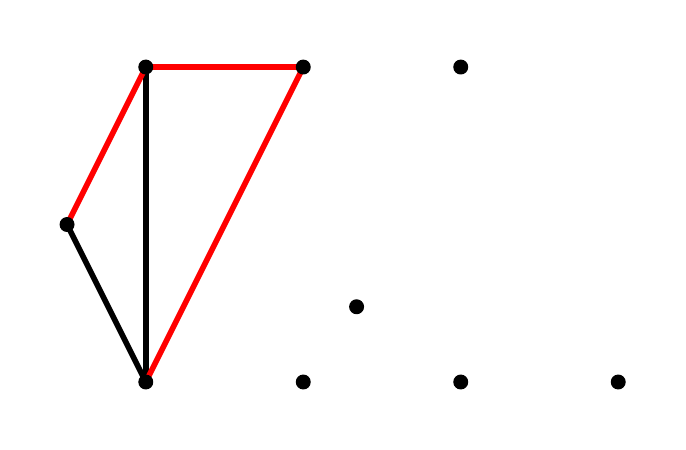
\begin{tikzpicture}[line cap=round,line join=round,x=1cm,y=1cm]
\clip(-.5,-.5) rectangle (7.5,4.5);
\draw [line width=2pt] (1,0)-- (1,4);
\draw [line width=2pt] (1,0)-- (0,2);
\draw [line width=2pt,color=ccqqqq] (1,4)-- (3,4);
\draw [line width=2pt,color=ccqqqq] (1,4)-- (0,2);
\draw [line width=2pt,color=ccqqqq] (1,0)-- (3,4);
\begin{scriptsize}
\draw [fill=black] (3,0) circle (2.5pt);
\draw [fill=black] (3.677138935355088,0.9555967043150745) circle (2.5pt);
\draw [fill=black] (1,0) circle (2.5pt);
\draw [fill=black] (1,4) circle (2.5pt);
\draw [fill=black] (0,2) circle (2.5pt);
\draw [fill=black] (3,4) circle (2.5pt);
\draw [fill=black] (5,0) circle (2.5pt);
\draw [fill=black] (5,4) circle (2.5pt);
\draw [fill=black] (7,0) circle (2.5pt);
\end{scriptsize}
\end{tikzpicture}}
\end{figure}
\end{frame}




\begin{frame}{A rotina \dymGraphReplace{}}
\begin{algorithm}[H]
\caption{\dymGraphReplace($G$,$u$,$v$,$\nivel$)}
\label{Algo:dymGraphReplace}
\begin{algorithmic}[1]
\For {$i$ $\gets$ $niv$ até $\lceil \lg n \rceil$}\label{Algo:dymGraphReplace:linha:primeira}
\State $T_v$ $\gets$  \treapGetRoot($F_i[v,v]$)
\State $T_u$ $\gets$  \treapGetRoot($F_i[u,u]$)
\If {\treapGetSize($T_v$) < \treapGetSize($T_u$)}\Comment{Garantimos que $|T_v|\geqslant |T_u|$}
\State $u$ $\leftrightarrow$ $v$
\State $T_u \leftrightarrow T_v$
\EndIf
\For {$xy$ em $T_u$ com \nivel = $i$}\label{Algo:dymGraphReplace:linha:moveTu}\Comment{Move $T_u$ para o nível $i-1$}
\State \nivel$[x,y]$ $\gets$ $i-1$ \label{Algo:dymGraphReplace:linha:moveTu2}
\State \dymForestAddEdge($G$.$F_{i-1}$, $x$, $y$) \label{Algo:dymGraphReplace:linha:moveTu3}
\EndFor
\For {$xy$ em $G$.$R_i$ com $x$ em $T_u$}\label{Algo:dymGraphReplace:linha:achaSub}\Comment{Procura substituta para $uv$}
\State \graphDel($G$.$R_i$, $x$, $y$)
\If {$y \in T_v$}\label{Algo:dymGraphReplace:linhayinTv}
\For {$j \gets i$ até $\lceil \lg n \rceil$}\label{Algo:dymGraphReplace:linha:inseresub}
\State \dymForestAddEdge($G$.$F_j$, $x$, $y$)
\EndFor
\State \Return
\Else
\State \nivel$[x,y]$ $\gets$ $i-1$ \label{Algo:dymGraphReplace:linha:rebaixar}
\State \graphAdd($G$.$R_{i-1}$, $x$, $y$) \label{Algo:dymGraphReplace:linha:rebaixar2}
\EndIf
\EndFor
\EndFor\label{Algo:dymGraphReplace:linha:ultima}
\end{algorithmic}
\end{algorithm}
\end{frame}


% --------------------------------------------------------------------- %
% Floresta maximal de peso mínimo em grafos planos ponderados dinâmicos %
% --------------------------------------------------------------------- %
\section[MSF plano]{Floresta maximal de peso mínimo em grafos planos ponderados dinâmicos}

\subsection{Definição do problema}
\begin{frame}{Floresta maximal de peso mínimo}
\begin{exampleblock}{O problema da floresta maximal de peso mínimo em grafos planos}
\begin{itemize}
\item \MSFCreate($n$): Cria e devolve um grafo plano ponderado~$G$ com $n$ vértices isolados.
\item \MSFaddEdge($G$, $e$, $u$, $e_u$, $v$, $e_v$, $w$): Insere em~$G$ uma nova aresta~$e$ com peso~$w$ ligando os vértices~$u$ e~$v$. A nova aresta~$e$ é sucessora das arestas~$e_u$ e~$e_v$ nas ordenações cíclicas de~$u$ e~$v$, respectivamente.
\item \MSFdelEdge($G$, $e$): Remove a aresta~$e$ de~$G$.
\item \MSFupdate($G$, $e$, $w$): Altera o peso da aresta~$e$ de~$G$ para o valor~$w$.
\item \MSFweight($G$): Devolve o peso de uma MSF de $G$.
\end{itemize}
\end{exampleblock}
\end{frame}

\begin{frame}{Grafo plano}
\begin{block}{Grafo plano}
Um \defi{grafo plano}~\cite{Diestel} é um par de conjuntos finitos $G = (V, E)$ com as seguintes propriedades:
\begin{enumerate}
\item $V\subset \R^2$;
\item Toda aresta é um arco entre dois vértices;
\item O interior de uma aresta não contém vértices nem intersecta outras arestas.
\end{enumerate}
\end{block}
\begin{minipage}[H]{0.4\textwidth}
\begin{tabular}{| c  c |} 
 \hline
 aresta & peso\\
 \hline
 $a$ & 2 \\ 
 \hline
$b$ & 7 \\
 \hline
$c$ & 3 \\
 \hline
$d$ & 1 \\
 \hline
$f$ & 2 \\
 \hline
$g$ & 4 \\
 \hline
\end{tabular}
\end{minipage}
\begin{minipage}[H]{0.4\textwidth}
\begin{figure}[H]
\scalebox{1}{
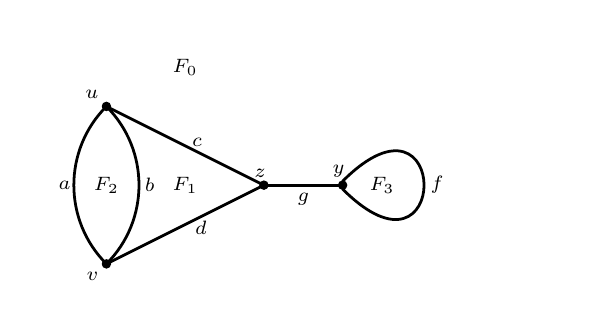
\begin{tikzpicture}[line cap=round,line join=round,x=1cm,y=1cm]
\clip(-1,-.5) rectangle (6,3);


\draw [line width=1pt] (0,0) to[in=-135,out=135,looseness=1]  (0,2); % v -- u
\draw [line width=1pt] (0,0) to[in=-45,out=45,looseness=1]  (0,2);   % v -- u
\draw [line width=1pt] (2,1) to  (0,0); % 4 -- 6
\draw [line width=1pt] (2,1) to  (0,2); % 4 -- 6
\draw [line width=1pt] (2,1) to  (3,1); % 4 -- 6
\draw [line width=1pt] (3,1.05) to[out=45,in=-45,looseness=50] (3,.95); % 4 -- 4


%\draw [line width=1pt] (1,2.5) to[out=-45,in=45,looseness=1] (1,1); % F0 -- F1
%\draw [line width=1pt] (1,2.5) to[out=20,in=-70,looseness=10] (1,1); % F0 -- F1
%\draw [line width=1pt] (1,2.5) to[out=170,in=180,looseness=2.5] (0,1); % F0 -- F2
%\draw [line width=1pt] (1,2.5) to[out=0,in=90,looseness=1] (2.5,1); % F0 -- F3
%\draw [line width=1pt] (1,1) to (0,1); % F1 -- F2




\begin{scriptsize}
\draw [fill=black] (0,2) circle (1.5pt);
\draw (0,2) node[anchor=south east] {$u$};


\draw [fill=black] (0,0) circle (1.5pt);
\draw (0,0) node[anchor=north east] {$v$};
\draw [fill=black] (2,1) circle (1.5pt);
\draw (1.95,1) node[anchor=south] {$z$};
\draw [fill=black] (3,1) circle (1.5pt);
\draw (2.95,1) node[anchor=south] {$y$};


%\draw [fill=black] (1,2.5) circle (1.5pt);
\draw (1,2.5) node {$F_0$};
%\draw [fill=black] (1,1) circle (1.5pt);
\draw (1,1) node {$F_1$};
%\draw [fill=black] (0,1) circle (1.5pt);
\draw (0,1) node {$F_2$};
%\draw [fill=black] (2.5,1) circle (1.5pt);
\draw (3.5,1) node {$F_3$};

%\draw (-0.3,1) node {$2$};
\draw (-0.53,1) node {$a$};

\draw (0.55,1.) node {$b$};
%\draw (0.53,1) node {$7$};

\draw (1.15,1.7) node[anchor=north] {$c$}; % u -- w
%\draw (1.05,1.5) node[anchor=north] {$3$}; % u -- w

\draw (1.2,.65) node[anchor=north] {$d$}; % v -- w
%\draw (1.35,.65) node[anchor=north] {$1$}; % v -- w

\draw (2.5,1) node[anchor=north] {$g$}; % v -- w
%\draw (2.5,.95) node[anchor=north] {$4$}; % v -- w


\draw (4.2,1) node {$f$}; % w -- w
%\draw (4.15,1) node {$2$}; % w -- w

\end{scriptsize}
\end{tikzpicture}

	}
\end{figure}
\end{minipage}

\end{frame}




\begin{frame}{Grafo dual}
\begin{block}{Grafo dual}
Dado um grafo plano~$G$, o grafo \defi{dual} de~$G$~\cite{Diestel} é o grafo $G^\star = (F,E^\star)$, onde
\begin{itemize}
\item $F$ é o conjunto de faces de~$G$;
\item $E^\star$ é o conjunto de arestas duais de~$G$.
\end{itemize}
\end{block}
\begin{figure}[H]
\scalebox{1.2}{
\centering
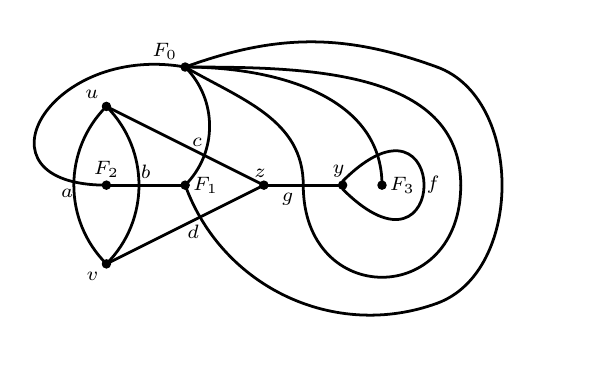
\begin{tikzpicture}[line cap=round,line join=round,x=1cm,y=1cm]
\clip(-1,-1) rectangle (6,3);


\draw [line width=1pt] (0,0) to[in=-135,out=135,looseness=1]  (0,2); % v -- u
\draw [line width=1pt] (0,0) to[in=-45,out=45,looseness=1]  (0,2);   % v -- u
\draw [line width=1pt] (2,1) to  (0,0); % 4 -- 6
\draw [line width=1pt] (2,1) to  (0,2); % 4 -- 6
\draw [line width=1pt] (2,1) to  (3,1); % 4 -- 6
\draw [line width=1pt] (3,1.05) to[out=45,in=-45,looseness=50] (3,.95); % 4 -- 4


\draw [line width=1pt] (1,2.5) to[out=-45,in=45,looseness=1] (1,1); % c: F0 -- F1
\draw [line width=1pt] (1,2.5) to[out=20,in=160,looseness=1] (4.2,2.5); % d: F0 -- F1
\draw [line width=1pt] (4.2,2.5) to[out=-20,in=20,looseness=1] (4.2,-.5); % d: F0 -- F1
\draw [line width=1pt] (1,1) to[out=-70,in=200,looseness=1] (4.2,-.5); % d: F0 -- F1


% laço F0 para F0
\draw [line width=1pt] (1,2.5) to[out=-30,in=90,looseness=1] (2.5,1); % F0 -- F1
\draw [line width=1pt] (2.5,1) to[out=-90,in=-90,looseness=2] (4.5,1); % F0 -- F1
\draw [line width=1pt] (1,2.5) to[out=0,in=90,looseness=1] (4.5,1); % F0 -- F1


\draw [line width=1pt] (1,2.5) to[out=170,in=180,looseness=2.5] (0,1); % F0 -- F2
\draw [line width=1pt] (1,2.5) to[out=0,in=90,looseness=1] (3.5,1); % F0 -- F3
\draw [line width=1pt] (1,1) to (0,1); % F1 -- F2




\begin{scriptsize}
\draw [fill=black] (0,2) circle (1.5pt);
\draw (0,2) node[anchor=south east] {$u$};


\draw [fill=black] (0,0) circle (1.5pt);
\draw (0,0) node[anchor=north east] {$v$};
\draw [fill=black] (2,1) circle (1.5pt);
\draw (1.95,1) node[anchor=south] {$z$};
\draw [fill=black] (3,1) circle (1.5pt);
\draw (2.95,1) node[anchor=south] {$y$};


\draw [fill=black] (1,2.5) circle (1.5pt);
\draw (1,2.5) node[anchor=south east] {$F_0$};
\draw [fill=black] (1,1) circle (1.5pt);
\draw (1,1) node[anchor=west] {$F_1$};
\draw [fill=black] (0,1) circle (1.5pt);
\draw (0,1) node[anchor=south] {$F_2$};
\draw [fill=black] (3.5,1) circle (1.5pt);
\draw (3.5,1) node[anchor=west] {$F_3$};

\draw (-0.5,1.05) node[anchor=north] {$a$};
%\draw (-0.5,1.1) node[anchor=north] {$2$};

\draw (0.5,1.35) node[anchor=north] {$b$};
%\draw (0.5,1.05) node[anchor=north] {$7$};

\draw (1.15,1.7) node[anchor=north] {$c$}; % u -- w
%\draw (1.4,1.7) node[anchor=north] {$3$}; % u -- w

\draw (1.1,.6) node[anchor=north] {$d$}; % v -- w
%\draw (1.2,.65) node[anchor=north] {$1$}; % v -- w

\draw (2.3,1) node[anchor=north] {$g$}; % v -- w
%\draw (2.3,.95) node[anchor=north] {$4$}; % v -- w

\draw (4.15,1) node {$f$}; % w -- w
%\draw (4.15,1) node {$2$}; % w -- w

\end{scriptsize}
\end{tikzpicture}

}
\label{fig:MSF-basico-1}
\end{figure}
\end{frame}


\begin{frame}{Grafo dual}
\begin{theorem}[\cite{EPPSTEIN-planar}]
\label{teo:MSFdual}
Seja~$T$ uma árvore geradora de um grafo plano conexo~$G$. O conjunto
$$
T^\star = \{e^\star:e\notin T\}
$$
é uma árvore geradora de~$G^\star$.
Além disso, se~$G$ for ponderado e adotarmos $w(e^\star) = w(e)$, então~$T$ será de peso mínimo em~$G$ se e somente se~$T^\star$ for de peso máximo em~$G^\star$ e vice versa.
\end{theorem}

\begin{figure}[H]
\scalebox{.6}{
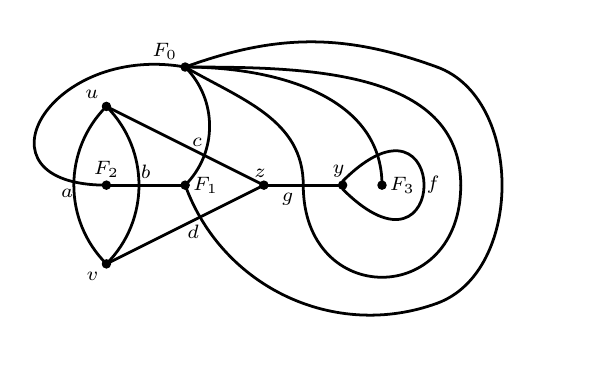
\begin{tikzpicture}[line cap=round,line join=round,x=1cm,y=1cm]
\clip(-1,-1) rectangle (6,3);


\draw [line width=1pt] (0,0) to[in=-135,out=135,looseness=1]  (0,2); % v -- u
\draw [line width=1pt] (0,0) to[in=-45,out=45,looseness=1]  (0,2);   % v -- u
\draw [line width=1pt] (2,1) to  (0,0); % 4 -- 6
\draw [line width=1pt] (2,1) to  (0,2); % 4 -- 6
\draw [line width=1pt] (2,1) to  (3,1); % 4 -- 6
\draw [line width=1pt] (3,1.05) to[out=45,in=-45,looseness=50] (3,.95); % 4 -- 4


\draw [line width=1pt] (1,2.5) to[out=-45,in=45,looseness=1] (1,1); % c: F0 -- F1
\draw [line width=1pt] (1,2.5) to[out=20,in=160,looseness=1] (4.2,2.5); % d: F0 -- F1
\draw [line width=1pt] (4.2,2.5) to[out=-20,in=20,looseness=1] (4.2,-.5); % d: F0 -- F1
\draw [line width=1pt] (1,1) to[out=-70,in=200,looseness=1] (4.2,-.5); % d: F0 -- F1


% laço F0 para F0
\draw [line width=1pt] (1,2.5) to[out=-30,in=90,looseness=1] (2.5,1); % F0 -- F1
\draw [line width=1pt] (2.5,1) to[out=-90,in=-90,looseness=2] (4.5,1); % F0 -- F1
\draw [line width=1pt] (1,2.5) to[out=0,in=90,looseness=1] (4.5,1); % F0 -- F1


\draw [line width=1pt] (1,2.5) to[out=170,in=180,looseness=2.5] (0,1); % F0 -- F2
\draw [line width=1pt] (1,2.5) to[out=0,in=90,looseness=1] (3.5,1); % F0 -- F3
\draw [line width=1pt] (1,1) to (0,1); % F1 -- F2




\begin{scriptsize}
\draw [fill=black] (0,2) circle (1.5pt);
\draw (0,2) node[anchor=south east] {$u$};


\draw [fill=black] (0,0) circle (1.5pt);
\draw (0,0) node[anchor=north east] {$v$};
\draw [fill=black] (2,1) circle (1.5pt);
\draw (1.95,1) node[anchor=south] {$z$};
\draw [fill=black] (3,1) circle (1.5pt);
\draw (2.95,1) node[anchor=south] {$y$};


\draw [fill=black] (1,2.5) circle (1.5pt);
\draw (1,2.5) node[anchor=south east] {$F_0$};
\draw [fill=black] (1,1) circle (1.5pt);
\draw (1,1) node[anchor=west] {$F_1$};
\draw [fill=black] (0,1) circle (1.5pt);
\draw (0,1) node[anchor=south] {$F_2$};
\draw [fill=black] (3.5,1) circle (1.5pt);
\draw (3.5,1) node[anchor=west] {$F_3$};

\draw (-0.5,1.05) node[anchor=north] {$a$};
%\draw (-0.5,1.1) node[anchor=north] {$2$};

\draw (0.5,1.35) node[anchor=north] {$b$};
%\draw (0.5,1.05) node[anchor=north] {$7$};

\draw (1.15,1.7) node[anchor=north] {$c$}; % u -- w
%\draw (1.4,1.7) node[anchor=north] {$3$}; % u -- w

\draw (1.1,.6) node[anchor=north] {$d$}; % v -- w
%\draw (1.2,.65) node[anchor=north] {$1$}; % v -- w

\draw (2.3,1) node[anchor=north] {$g$}; % v -- w
%\draw (2.3,.95) node[anchor=north] {$4$}; % v -- w

\draw (4.15,1) node {$f$}; % w -- w
%\draw (4.15,1) node {$2$}; % w -- w

\end{scriptsize}
\end{tikzpicture}

}
\scalebox{1}{
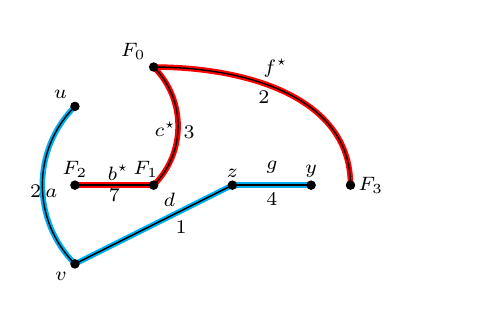
\begin{tikzpicture}[line cap=round,line join=round,x=1cm,y=1cm]
\clip(-.6,-.5) rectangle (5,3);


\draw [line width=2pt,color=cyan] (0,0) to[in=-135,out=135,looseness=1]  (0,2); % v -- u
\draw [line width=.5pt] (0,0) to[in=-135,out=135,looseness=1]  (0,2); % v -- u
%\draw [line width=1pt] (0,0) to[in=-45,out=45,looseness=1]  (0,2);   % v -- u
\draw [line width=2pt,color=cyan] (2,1) to  (0,0); % 4 -- 6
\draw [line width=.5pt] (2,1) to  (0,0); % 4 -- 6
\draw [line width=2pt,color=cyan] (2,1) to  (3,1); % 4 -- 6
\draw [line width=.5pt] (2,1) to  (3,1); % 4 -- 6
%\draw [line width=1pt] (2,1) to  (0,2); % 4 -- 6
%\draw [line width=1pt] (2,1.05) to[out=45,in=-45,looseness=50] (2,.95); % 4 -- 4

\draw [line width=2pt,color=red] (1,2.5) to[out=-45,in=45,looseness=1] (1,1); % F0 -- F1
\draw [line width=.5pt] (1,2.5) to[out=-45,in=45,looseness=1] (1,1); % F0 -- F1
%\draw [line width=1pt] (1,2.5) to[out=20,in=-70,looseness=10] (1,1); % F0 -- F1
%\draw [line width=1pt] (1,2.5) to[out=170,in=180,looseness=2.5] (0,1); % F0 -- F2
\draw [line width=2pt,color=red] (1,2.5) to[out=0,in=90,looseness=1] (3.5,1); % F0 -- F3
\draw [line width=.5pt] (1,2.5) to[out=0,in=90,looseness=1] (3.5,1); % F0 -- F3
\draw [line width=2pt,color=red] (1,1) to (0,1); % F1 -- F2
\draw [line width=.5pt] (1,1) to (0,1); % F1 -- F2

\begin{scriptsize}
\draw [fill=black] (0,2) circle (1.5pt);
\draw (0,2) node[anchor=south east] {$u$};


\draw [fill=black] (0,0) circle (1.5pt);
\draw (0,0) node[anchor=north east] {$v$};
\draw [fill=black] (2,1) circle (1.5pt);
\draw (2,1) node[anchor=south] {$z$};
\draw [fill=black] (3,1) circle (1.5pt);
\draw (3,1) node[anchor=south] {$y$};


\draw [fill=black] (1,2.5) circle (1.5pt);
\draw (1,2.5) node[anchor=south east] {$F_0$};
\draw [fill=black] (1,1) circle (1.5pt);
\draw (.9,1) node[anchor=south] {$F_1$};
\draw [fill=black] (0,1) circle (1.5pt);
\draw (0,1) node[anchor=south] {$F_2$};
\draw [fill=black] (3.5,1) circle (1.5pt);
\draw (3.5,1) node[anchor=west] {$F_3$};


\draw (-0.3,1.05) node[anchor=north] {$a$};
\draw (-0.5,1.1) node[anchor=north] {$2$};

\draw (0.55,1.35) node[anchor=north] {$b^\star$};
\draw (0.5,1.05) node[anchor=north] {$7$};

\draw (1.15,1.9) node[anchor=north] {$c^\star$}; % u -- w
\draw (1.45,1.85) node[anchor=north] {$3$}; % u -- w

\draw (1.2,1) node[anchor=north] {$d$}; % v -- w
\draw (1.35,.65) node[anchor=north] {$1$}; % v -- w

\draw (2.5,1.4) node[anchor=north] {$g$}; % v -- w
\draw (2.5,1) node[anchor=north] {$4$}; % v -- w

\draw (2.55,2.7) node[anchor=north] {$f^\star$}; % w -- w
\draw (2.4,2.3) node[anchor=north] {$2$}; % w -- w

\end{scriptsize}
\end{tikzpicture}

}
\end{figure}
\end{frame}



\begin{frame}{Grafo dual}
\begin{minipage}[H]{0.4\textwidth}
\centering
\begin{tabular}{| c  c |} 
 \hline
 vértices & pesos\\
 \hline
 $\hat a$, $\hat a_1$, $\hat a_3$ & 2 \\ 
 \hline
 $\hat b$, $\hat b_0$, $\hat b_2$ & 7 \\
 \hline
 $\hat c$, $\hat c_0$, $\hat c_2$ & 3 \\
 \hline
 $\hat d$, $\hat d_0$, $\hat d_2$ & 2 \\
 \hline
 $\hat f$, $\hat f_1$, $\hat f_3$ & 1 \\
 \hline
 $\hat g$, $\hat g_1$, $\hat g_3$ & 4 \\
 \hline
 $\hat u$, $\hat v$, $\hat y$, $\hat z$ & $-\infty$ \\
 \hline
 $\hat F_0$, $\hat F_1$, $\hat F_2$, $\hat F_3$ & $\infty$ \\
 \hline
\end{tabular}
\end{minipage}
\hfill
\begin{minipage}[H]{0.5\textwidth}
    \centering
\scalebox{.6}{
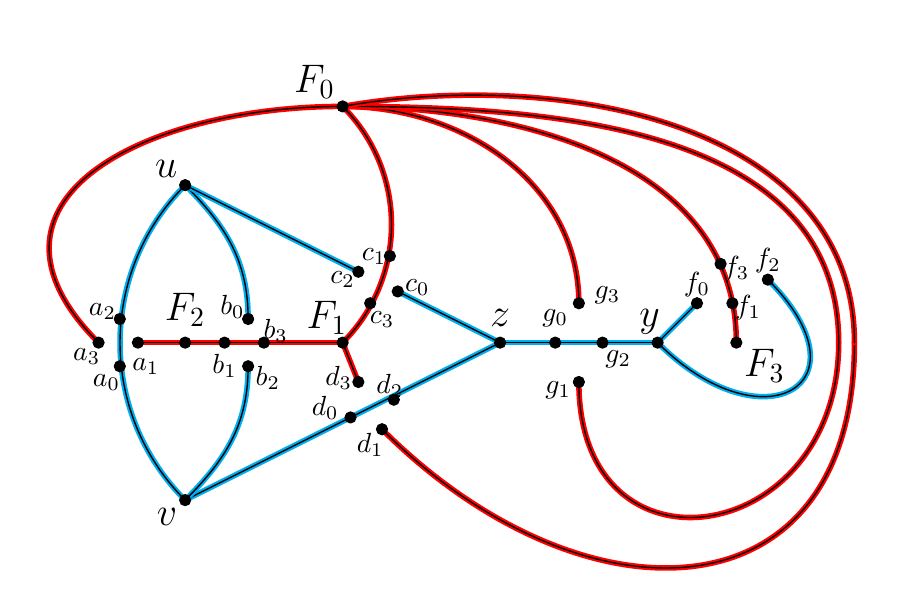
\begin{tikzpicture}[line cap=round,line join=round,x=1cm,y=1cm]
\clip(-2,-1) rectangle (9,6);

\draw [line width=2pt,color=cyan] (0,0) to[in=-135,out=135,looseness=1]  (0,4); % v -- u
\draw [line width=.5pt] (0,0) to[in=-135,out=135,looseness=1]  (0,4); % v -- u
%\draw [line width=1pt] (0,0) to[in=-45,out=45,looseness=1]  (0,4);   % v -- u

\draw [line width=2pt,color=cyan] (4,2) to  (0,0); % 4 -- 6
\draw [line width=.5pt] (4,2) to  (0,0); % 4 -- 6
%\draw [line width=1pt] (4,2) to  (0,4); % 4 -- 6
%\draw [line width=1pt] (4,2.05) to[out=45,in=-45,looseness=100] (4,1.95); % w -- w

\draw [line width=2pt,color=red] (2,5) to[out=-45,in=45,looseness=1] (2,2); % F0 -- F1
\draw [line width=.5pt] (2,5) to[out=-45,in=45,looseness=1] (2,2); % F0 -- F1
%\draw [line width=1pt] (2,5) to[out=20,in=-70,looseness=7.5] (2,2); % F0 -- F1
%\draw [line width=1pt] (2,5) to[out=170,in=180,looseness=2] (0,2); % F0 -- F2
\draw [line width=2pt,color=red] (2,5) to[out=0,in=90,looseness=1] (7,2); % F0 -- F3
\draw [line width=.5pt] (2,5) to[out=0,in=90,looseness=1] (7,2); % F0 -- F3

\draw [line width=2pt,color=red] (2,2) to (0,2); % F1 -- F2
\draw [line width=.5pt] (2,2) to (0,2); % F1 -- F2

\draw [line width=2pt,color=red] (2,5) to[out=0,in=90,looseness=1] (5,2.5); % F0 -- F0
\draw [line width=.5pt] (2,5) to[out=0,in=90,looseness=1] (5,2.5); % F0 -- F0


%F0 -- e1
\draw [line width=2pt,color=red] (2,5) to[out=0,in=90,looseness=1] (8.3,2); % F0 -- F0
\draw [line width=2pt,color=red] (8.3,2) to[out=-90,in=-90,looseness=2] (5, 1.5); % F0 -- F0
\draw [line width=.5pt] (2,5) to[out=0,in=90,looseness=1] (8.3,2); % F0 -- F0
\draw [line width=.5pt] (8.3,2) to[out=-90,in=-90,looseness=2] (5, 1.5); % F0 -- F0

\begin{scriptsize}

% Aresta a
\draw [line width=2pt,color=red] (0,2) to  (-.6,2); 
\draw [line width=.5pt] (0,2) to  (-.6,2); 
\draw [line width=2pt,color=red] (-1.1,2) to[out=135,in=180,looseness=1.5]  (2,5);   % v -- u
\draw [line width=.5pt] (-1.1,2) to[out=135,in=180,looseness=1.5]  (2,5);   % v -- u
\draw (-1,1.7) node[anchor=north] {{\normalsize $a_0$}};
\draw [fill=black] (-.83,1.7) circle (2pt);
\draw (-.5,1.9) node[anchor=north] {{\normalsize $a_1$}};
\draw [fill=black] (-.6,2) circle (2pt);
\draw (-1.05,2.6) node[anchor=north] {{\normalsize $a_2$}};
\draw [fill=black] (-.83,2.3) circle (2pt);
\draw (-1.25,2.03) node[anchor=north] {{\normalsize $a_3$}};
\draw [fill=black] (-1.1,2) circle (2pt);



% Aresta b
\draw [line width=2pt,color=cyan] (0,0) to[in=-90,out=45,looseness=1]  (.8,1.7);   % v -- u
\draw [line width=.5pt] (0,0) to[in=-90,out=45,looseness=1]  (.8,1.7);   % v -- u

\draw [line width=2pt,color=cyan] (0,4) to[out=-45,in=90,looseness=1]  (.8,2.3);   % v -- u
\draw [line width=.5pt] (0,4) to[out=-45,in=90,looseness=1]  (.8,2.3);   % v -- u

\draw (.6,2.7) node[anchor=north] {{\normalsize $b_0$}};
\draw [fill=black] (.8,2.3) circle (2pt);
\draw (.5,1.95) node[anchor=north] {{\normalsize $b_1$}};
\draw [fill=black] (.5,2) circle (2pt);
\draw (1.05,1.8) node[anchor=north] {{\normalsize $b_2$}};
\draw [fill=black] (.8,1.7) circle (2pt);
\draw (1.15,2.4) node[anchor=north] {{\normalsize $b_3$}};
\draw [fill=black] (1,2) circle (2pt);



% Aresta c

\draw [line width=2pt,color=cyan] (0,4) to  (2.2,2.9);   
\draw [line width=.5pt] (0,4) to  (2.2,2.9);   
\draw [line width=2pt,color=cyan] (2.7,2.65) to  (4,2);   
\draw [line width=.5pt] (2.7,2.65) to  (4,2);   

\draw (2.95,2.9) node[anchor=north] {{\normalsize $c_0$}}; % u -- w
\draw [fill=black] (2.7,2.65) circle (2pt);
\draw (2.4,3.3) node[anchor=north] {{\normalsize $c_1$}}; % u -- w
\draw [fill=black] (2.6,3.1) circle (2pt);
\draw (2,3) node[anchor=north] {{\normalsize $c_2$}}; % u -- w
\draw [fill=black] (2.2,2.9) circle (2pt);
\draw (2.5,2.5) node[anchor=north] {{\normalsize $c_3$}}; % u -- w
\draw [fill=black] (2.35,2.5) circle (2pt);



% Aresta d
\draw [line width=2pt,color=red] (2,2) to  (2.2,1.5);   
\draw [line width=.5pt] (2,2) to  (2.2,1.5);   

\draw [line width=2pt,color=red] (2.5,.9) to[out=-45,in=-90,looseness=1.5]  (8.5,2);   
\draw [line width=.5pt] (2.5,.9) to[out=-45,in=-90,looseness=1.5]  (8.5,2);   
\draw [line width=2pt,color=red] (2,5) to[out=10,in=90,looseness=1]  (8.5,2);   
\draw [line width=.5pt] (2,5) to[out=10,in=90,looseness=1]  (8.5,2);   



\draw (2.05,1.175) node[anchor=east] {{\normalsize $d_0$}}; % v -- w
\draw [fill=black] (2.1,1.05) circle (2pt);

\draw (2.35,.95) node[anchor=north] {{\normalsize $d_1$}}; % v -- w
\draw [fill=black] (2.5,.9) circle (2pt);

\draw (2.6,1.7) node[anchor=north] {{\normalsize $d_2$}}; % v -- w
\draw [fill=black] (2.65,1.275) circle (2pt);

\draw (1.95,1.8) node[anchor=north] {{\normalsize $d_3$}}; % v -- w
\draw [fill=black] (2.2,1.5) circle (2pt);

% Aresta e
\draw [line width=2pt,color=cyan] (4,2) to  (6,2);   
\draw [line width=.5pt] (4,2) to  (6,2);   

\draw (4.7,2.1) node[anchor=south] {{\normalsize $g_0$}}; % v -- w
\draw [fill=black] (4.7,2) circle (2pt);
\draw (5,1.4) node[anchor=east] {{\normalsize $g_1$}}; % v -- w
\draw [fill=black] (5,1.5) circle (2pt);
\draw (5.5,2) node[anchor=north] {{\normalsize $g_2$}}; % v -- w
\draw [fill=black] (5.3,2) circle (2pt);
\draw (5.1,2.6) node[anchor=west] {{\normalsize $g_3$}}; % v -- w
\draw [fill=black] (5,2.5) circle (2pt);



% Aresta f

\draw [line width=2pt,color=cyan] (6,2) to  (6.5,2.5);   
\draw [line width=.5pt] (6,2) to  (6.5,2.5);   
\draw [line width=2pt,color=cyan] (6,2) to[out=-45,in=-45,looseness=3]  (7.4,2.8);   
\draw [line width=.5pt] (6,2) to[out=-45,in=-45,looseness=3]  (7.4,2.8);   

\draw (6.5,3) node[anchor=north] {{\normalsize $f_0$}}; % w -- w
\draw [fill=black] (6.5,2.5) circle (2pt);
\draw (7.15,2.7) node[anchor=north] {{\normalsize $f_1$}}; % w -- w
\draw [fill=black] (6.95,2.5) circle (2pt);
\draw (7.4,3.3) node[anchor=north] {{\normalsize $f_2$}}; % w -- w
\draw [fill=black] (7.4,2.8) circle (2pt);
\draw (7,3.2) node[anchor=north] {{\normalsize $f_3$}}; % w -- w
\draw [fill=black] (6.8,3) circle (2pt);



\draw [fill=black] (0,4) circle (2pt);
\draw (0,4) node[anchor=south east] {{\Large $u$}};

\draw [fill=black] (0,0) circle (2pt);
\draw (0,0) node[anchor=north east] {{\Large $v$}};
\draw [fill=black] (4,2) circle (2pt);
\draw (4,2.1) node[anchor=south] {{\Large $z$}};
\draw [fill=black] (6,2) circle (2pt);
\draw (5.9,2) node[anchor=south] {{\Large $y$}};

\draw [fill=black] (2,5) circle (2pt);
\draw (2,5) node[anchor=south east] {{\Large $F_0$}};
\draw [fill=black] (2,2) circle (2pt);
\draw (1.8,2) node[anchor=south] {{\Large $F_1$}};
\draw [fill=black] (0,2) circle (2pt);
\draw (0,2.1) node[anchor=south] {{\Large $F_2$}};
\draw [fill=black] (7,2) circle (2pt);
\draw (7,1.7) node[anchor=west] {{\Large $F_3$}};


\end{scriptsize}
\end{tikzpicture}

}
\end{minipage}
\end{frame}

\begin{frame}{Grafo dual}
\end{frame}

\begin{frame}{Grafo dual}
\end{frame}

\begin{frame}{Grafo dual}
\end{frame}

\begin{frame}{Grafo dual}
\end{frame}

\begin{frame}{Grafo dual}
\end{frame}

\subsection{Árvores dinâmicas planas}
\begin{frame}{Árvores Dinâmicas Planas}
\begin{exampleblock}{Biblioteca ADP}
\begin{itemize}
\item \LCOMakeOcto($e$, $w$): Recebe um identificador~$e$ e um peso~$w$ e cria e retorna uma óctupla de nós de ADP associados a~$e$ com peso~$w$.
\item \LCODestroyOcto($H$, $e$): Recebe uma tabela de símbolos~$H$ e um identificador~$e$ e desaloca a óctupla associada a~$e$ da memória.

\item \LCOConnected($p$, $q$): Retorna verdadeiro se os nós~$p$ e~$q$ estiverem na mesma ADP e falso caso contrário.
\item \LCOFindNode($p$): Recebe um nó $p$ e retorna o vértice da~$\hat F$ que contêm $p$ em sua ordem cíclica.

\item \LCOAddCost($p$, $w$): Atribui o peso~$w$ ao vértice que contém $p$ em sua ordem cíclica.
\item \LCOMax($p$, $q$): Retorna o nó de peso máximo no percurso entre os nós~$p$ e~$q$.
Essa operação assume que $p$ e~$q$ são nós da mesma ADP.
\item \LCOMin($p$, $q$): Retorna o nó de peso mínimo no percurso entre os nós~$p$ e~$q$.
Essa operação assume que~$p$ e~$q$ são nós da mesma ADP.
\item \LCOCycle($p$): Permuta ciclicamente $D(u)$ de forma que o nó~$p$ seja o último na ordem.
Se a ordem inicial tem forma $\alpha p \beta$, então a ordem resultante é $\beta\alpha p$.
\item \treapPredecessor($p$): Retorna o predecessor do nó~$p$ na ordem cíclica.
\end{itemize}
\end{exampleblock}
\end{frame}

\subsection{Resolvendo MSF com ADPs}
\subsection{Implementação de árvores dinâmicas planas}


\section{O limitante inferior de~$\Omega(\lg n)$}
\subsection{O modelo de computação cell-probe}
\subsection{Verificação de soma parcial em~$S_k$}
\subsection[Redução do VSP$S_k$ para conexidade em grafos dinâmicos]{Redução do problema VSP$S_k$ para conexidade em grafos dinâmicos}
\subsection{Limitante inferior para conexidade em grafos dinâmicos}


\section{Bibliografia}
\begin{frame}[allowframebreaks]
\frametitle{Bibliografia}
\bibliographystyle{plain}
    \bibliography{bib.bib}
\end{frame}

\end{document}
